Trong quá trình hoạt động kinh doanh, không phải mọi doanh nghiệp đều giữ nguyên mô hình kinh doanh được đưa ra ban đầu. Việc chuyển đổi mô hình kinh doanh là điều cần thiết, giúp các doanh nghiệp có thể phát triển linh hoạt và tồn tại.

\begin{example}

    \begin{itemize}

        \item Google bắt đầu như công cụ tìm kiếm trực tuyến, nhưng sau đó đã mở rộng và thay đổi mô hình kinh doanh qua nhiều dịch vụ và sản phẩm khác nhau như: Dịch vụ đám mây Google Cloud Platform, Dịch vụ thư điện tử Gmail, Dịch vụ bản đồ Google Maps, Dịch vụ lưu trữ tập tin Google Drive, \dots

        \item Amazon từ hiệu sách trực tuyến đã trở thành thị trường cho nhà cung cấp khác như: Thương mại điện tử, Dịch vụ đám mây Amazon Web Services (AWS), \dots

    \end{itemize}

\end{example}

\begin{figure}[H]

    \centering

    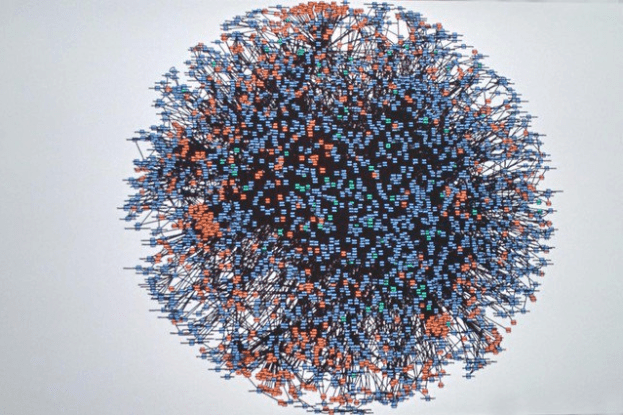
\includegraphics[scale = 0.5]{pictures/_kien_truc_vi_dich_vu_cua_amazon/main.png}

    \caption{Kiến trúc vi dịch vụ của Amazon}

\end{figure}

Đối với những doanh nghiệp không chuyển đổi kinh doanh sẽ không thể tồn tại.

\begin{example} Gần đây, dịch vụ giao đồ ăn Baemin đã rời khỏi thị trường Việt Nam cũng do sức ép từ các đối thủ khác khiến Baemin khó cạnh tranh trong mảng kinh doanh cốt lõi là giao đồ ăn. Các đối thủ này không chỉ cung cấp dịch vụ giao đồ ăn mà còn có đặt xe, giao hàng, \dots

\end{example}

\begin{figure}[H]

    \centering

    
\includegraphics[scale = 0.5]{pictures/_baemin/main.png}

    \caption{Dịch vụ giao đồ ăn Baemin đã rời khỏi thị trường Việt Nam}

\end{figure}


$\Rightarrow$  Hiện nay, các tổ chức doanh nghiệp có nhu cầu chuyển đổi kinh doanh để có thể tồn tại và phát triển khi thị trường thay đổi. Từ đó, đáp ứng nhu cầu của khách hàng, mang lại ưu thế cạnh tranh so với các đối thủ.       Do đó, các doanh nghiệp cần hệ thống chuyển đổi nhanh chóng để đáp ứng nhu cầu của mô hình kinh doanh,  đặt ra thách thức đối với kiến trúc phần mềm.


Kiến trúc nguyên khối đã phục vụ hiệu quả trong quá khứ, nhưng kiến trúc này bắt đầu gặp khó khăn khi đối mặt với sự phức tạp, khả năng mở rộng và khả năng đáp ứng linh hoạt.   Kiến trúc vi dịch vụ là giải pháp cho những thách thức trên. Kiến trúc vi dịch vụ chia dự án thành những dịch vụ nhỏ độc lập, mỗi dịch vụ chịu trách nhiệm về một chức năng cụ thể     tăng tính linh hoạt và chuyển đổi nhanh chóng.


